%! TeX program = xelatex
%======================PROPIEDADES DEL DOCUMENTO======================================
\documentclass[12pt,a4paper]{article}

%==========================PAQUETES======================================
\usepackage[spanish, es-noshorthands]{babel} 
\usepackage{listings}
\usepackage{subcaption}
\usepackage{graphicx}
\usepackage{float}
\usepackage{titlesec}  
\usepackage[section]{placeins}
\usepackage{anysize}
\usepackage{fontspec} % Para usar Times New Roman
\usepackage[dvipsnames]{xcolor}
\usepackage{amsmath}
\usepackage{siunitx}
\usepackage{circuitikz}
\usepackage{lipsum}
\usepackage{cite}
\usepackage{multirow}
\usepackage{booktabs}
\usepackage{colortbl}
\usepackage{bigstrut}
\usepackage{comment}
\usepackage{fancyhdr}  
\usepackage{setspace} % Para el interlineado
\usepackage{tabularx}
\usepackage{karnaugh-map}
\usepackage{hyperref}

%=========================================
%========== CODIGO ======================
%=========================================

\lstdefinestyle{mystyle}{
    backgroundcolor=\color{backcolour},
    commentstyle=\color{codegreen},
    keywordstyle=\color{magenta},
    numberstyle=\tiny\color{codegray},
    stringstyle=\color{codepurple},
    basicstyle=\ttfamily\footnotesize,
    breakatwhitespace=false,         
    breaklines=true,                 
    captionpos=b,                    
    keepspaces=true,                 
    numbers=none,                    
    numbersep=5pt,                  
    showspaces=false,                
    showstringspaces=false,
    showtabs=false,                  
    tabsize=2
}

\definecolor{codegreen}{rgb}{0,0.6,0}
\definecolor{codegray}{rgb}{0.5,0.5,0.5}
\definecolor{codepurple}{rgb}{0.58,0,0.82}
\definecolor{backcolour}{rgb}{0.95,0.95,0.95}

\lstset{style=mystyle}


%==========================FUENTE Y ESTILO======================================
\setmainfont{Times New Roman} % Fuente principal
\renewcommand{\baselinestretch}{1.0} % Interlineado sencillo

%==========================COLORES======================================
\definecolor{azulFuerte}{RGB}{0, 0, 120}
\definecolor{rojoUPIITA}{RGB}{180,0,0}
\definecolor{Amarillo}{RGB}{227,162,7}
\definecolor{Verde}{RGB}{13,171,49}

%============================Formato para las secciones===========================
% Quitar numeración en secciones
\titleformat{\section}
  {\bfseries\color{Amarillo}\Large}{}{0em}{}

% ===============================MÁRGENES=========================================
\marginsize{25mm}%izquierda
{25mm} %derecha
{15mm} %arriba
{15mm} %abajo
\setlength{\headheight}{15pt}

%======================== ENCABEZADO==============================================
\pagestyle{empty} % Quitar numeración de páginas y encabezados

%=========================INICIO DEL DOCUMENTO=====================================
\begin{document}

%===============================PORTADA==============================================
% Línea superior con UPIITA a la izquierda y DLP a la derecha
\noindent
\makebox[\textwidth]{%
    \textbf{UPIITA-IPN}%
    \hfill%
    \textcolor{rojoUPIITA}{\textbf{Dispositivos Lógicos Programables}}%
}

% Bloque inferior: alumnos a la izquierda, logo a la derecha
\vspace{5mm}

\noindent
\begin{minipage}{0.6\textwidth}
    \raggedright% Alinea a la izquierda este bloque
    \textbf{Práctica 01: Nombre de la práctica}\\[2mm]
    \textbf{Alumno 1:} Flores Oropeza Osvaldo\\
    \textbf{Alumno 2:} Ramirez Aguilar Victor Saul\\
    \textbf{Alumno 3:} Reyes Lira Alejandro\\
    \textbf{Grupo:} 2MV11
\end{minipage}%
\hfill
\begin{minipage}{0.35\textwidth}
    \raggedleft% Alinea a la derecha este bloque
    
\includegraphics[width=0.65\textwidth]{logos/logo_Kin.jpeg}
\end{minipage}

\vspace{10mm}

%================================DOCUMENTO===========================================


\section{Resumen}
%! TEX root = C:\Users\osval\OneDrive - Instituto Politecnico Nacional\Codigos\Programacion\DLP\Practica_1\main.tex

La práctica consiste en el uso de lenguajes de descripción de hardware (VHDL y Verilog) para implementar y simular circuitos digitales en una tarjeta de desarrollo FPGA. Se trabajan tanto circuitos combinacionales como secuenciales: funciones lógicas básicas, un registro de 8 bits con flip-flops tipo D, un contador binario ascendente/descendente de 4 bits con salida a display de 7 segmentos, y generadores de sonido. Finalmente, se integran los distintos módulos en un Top Level Design (TLD), que concentra todas las funciones en un solo proyecto. El objetivo es que el estudiante se familiarice con el proceso completo de diseño digital: programación, simulación, implementación y prueba en hardware real.

\section{Abstract}
%! TEX root = C:\Users\osval\OneDrive - Instituto Politecnico Nacional\Codigos\Programacion\DLP\Practica_1\main.tex

The practice focuses on the use of Hardware Description Languages (VHDL and Verilog) to implement and simulate digital circuits on an FPGA development board. Both combinational and sequential circuits are developed: basic logic functions, an 8-bit register based on D flip-flops, a 4-bit up/down binary counter with a 7-segment display output, and sound generators. Finally, all the modules are integrated into a Top Level Design (TLD), which combines every function into a single project. The goal is to help students become familiar with the complete digital design flow: programming, simulation, implementation, and testing on real hardware.

\section{Resumo}
%! TEX root = C:\Users\osval\OneDrive - Instituto Politecnico Nacional\Codigos\Programacion\DLP\Practica_1\main.tex

A prática consiste no uso de linguagens de descrição de hardware (VHDL e Verilog) para implementar e simular circuitos digitais em uma placa de desenvolvimento FPGA. São trabalhados circuitos combinacionais e sequenciais: funções lógicas básicas, um registrador de 8 bits com flip-flops tipo D, um contador binário crescente/decrescente de 4 bits com saída em display de 7 segmentos e geradores de som. Por fim, todos os módulos são integrados em um Top Level Design (TLD), que reúne todas as funções em um único projeto. O objetivo é que o aluno se familiarize com todo o processo de projeto digital: programação, simulação, implementação e teste em hardware real.

%! TEX root = C:\Users\osval\OneDrive - Instituto Politecnico Nacional\Codigos\Programacion\DLP\Practica_1\main.tex

\newpage
\textbf{Tabla de Contenido.}

\begin{table}[H]
    \centering
    % Table generated by Excel2LaTeX from sheet 'Hoja1'
\begin{tabular}{|c|c|c|c|c|}
\hline
Puntos & Codigo VHDL & Codigo Verilog & Fotos  & Simulación \bigstrut\\
\hline
1. Funciones &   &   &   &  \bigstrut\\
\hline
2. Registro 8 bits &   &   &   &  \bigstrut\\
\hline
3. Contador &   &   &   &  \bigstrut\\
\hline
4. Sirenas & \cellcolor[rgb]{ .816,  .816,  .816} &   &   & \cellcolor[rgb]{ .816,  .816,  .816} \bigstrut\\
\hline
5. TLD  &   &   &   & \cellcolor[rgb]{ .816,  .816,  .816} \bigstrut\\
\hline
\multicolumn{1}{|p{7.665em}|}{6. Encoder, Pmod, RS232} &   & \cellcolor[rgb]{ .816,  .816,  .816} &   & \cellcolor[rgb]{ .816,  .816,  .816} \bigstrut\\
\hline
CH & \cellcolor[rgb]{ .816,  .816,  .816} & \cellcolor[rgb]{ .816,  .816,  .816} & \cellcolor[rgb]{ .816,  .816,  .816} & \cellcolor[rgb]{ .816,  .816,  .816} \bigstrut\\
\hline
\end{tabular}%
    \caption{Tabla de contenido}
    \label{tab:Tabla de contenido}
\end{table}

\section{Pre-reporte}
%! TEX root = C:\Users\osval\OneDrive - Instituto Politecnico Nacional\Codigos\Programacion\DLP\Practica_1\main.tex

Como parte del pre-reporte solicitado, se presentan los siguientes puntos investigados:

\subsection*{Lenguajes de Descripción de Hardware (HDL)}
Los lenguajes de descripción de hardware (HDL, por sus siglas en inglés) permiten describir el comportamiento y la estructura de sistemas digitales. Los más utilizados son:
\begin{itemize}
    \item \textbf{VHDL}: Lenguaje robusto, fuertemente tipado y muy usado en la industria aeroespacial y militar. Facilita el modelado en distintos niveles de abstracción (comportamental, RTL, estructural).
    \item \textbf{Verilog}: Lenguaje más simple y con sintaxis similar a C. Es ampliamente empleado en aplicaciones industriales y académicas, especialmente en diseño de lógica digital.
\end{itemize}
Ambos lenguajes permiten la simulación, verificación, síntesis e implementación de circuitos digitales en CPLDs y FPGAs.

\subsection*{CPLD y FPGA}
\begin{itemize}
    \item \textbf{CPLD (Complex Programmable Logic Device)}: Son dispositivos lógicos programables de mediana capacidad, con arquitectura basada en macroceldas. Son adecuados para implementar lógica combinacional y secuencial de menor escala.
    \item \textbf{FPGA (Field Programmable Gate Array)}: Dispositivos programables con gran cantidad de bloques lógicos configurables, memoria interna y recursos adicionales (DSPs, PLLs, etc.). Permiten implementar desde sistemas digitales simples hasta procesadores completos.
\end{itemize}

\subsection*{Circuitos Externos Requeridos}
Para el desarrollo de la práctica se requieren algunos circuitos adicionales:
\begin{itemize}
    \item \textbf{Etapa de potencia de audio}: Amplificador de al menos 3W para excitar una bocina de 4 u 8 ohms.
    \item \textbf{Fuente de alimentación externa}: Regulada para garantizar un funcionamiento estable de los módulos adicionales.
    \item \textbf{Periféricos}: PmodALS (sensor de luz), encoder rotatorio y conexiones para RS232, dependiendo de las actividades a desarrollar.
\end{itemize}

\subsection*{Metodología General}
El flujo de trabajo típico en la práctica consiste en:
\begin{enumerate}
    \item Creación del proyecto en el software de desarrollo (ISE, Vivado o Quartus).
    \item Escritura del código HDL en VHDL y Verilog.
    \item Simulación y verificación funcional en el simulador integrado.
    \item Síntesis e implementación del diseño.
    \item Generación del archivo de programación (*.bit o *.jed).
    \item Programación de la FPGA y verificación física de los resultados.
\end{enumerate}

\section{Introducción}
%! TEX root = C:\Users\osval\OneDrive - Instituto Politecnico Nacional\Codigos\Programacion\DLP\Practica_1\main.tex

En esta práctica se busca que el estudiante se familiarice con el uso de lenguajes de descripción de hardware (HDL), principalmente VHDL y Verilog, para implementar y simular circuitos digitales dentro de una tarjeta de desarrollo FPGA. 

Los circuitos a desarrollar incluyen tanto sistemas combinacionales como secuenciales: funciones lógicas básicas a partir de una tabla de verdad, un registro de 8 bits basado en flip-flops tipo D, un contador binario ascendente/descendente de 4 bits con salida a un display de 7 segmentos, así como generadores de sonido (sirenas). 

Finalmente, se integrarán los módulos en un \textit{Top Level Design} (TLD), el cual permite concentrar todas las funciones en un único diseño jerárquico. De esta forma, el alumno recorre todo el flujo de diseño digital: codificación, simulación, síntesis, implementación y prueba en hardware real, aplicando conocimientos teóricos a aplicaciones prácticas.

\subsection*{Registro 8 bits}

Un registro de 8 bits es un circuito electrónico para el almacenamiento y proceso de datos de 8 bits.

Para el desarrollo del registro de 8 bits se va a tomar como base el uso de un flip flop tipo D (Figura: \ref{fig:FF-D}) el cual funciona para guardar un bit de la entrada D en el momento en el que exista un flanco de subida en la entrada del CLK, y este se va a mostrar en la salida Q, y en la salida Q' se va a mostrar el estado en el que se encontraba la entrada D antes del cambio del flanco de subida en el CLK. 

\begin{figure}[H]
    \centering
        \resizebox{0.2\linewidth}{!}{
    \begin{tikzpicture}
	% Paths, nodes and wires:
	\node[flipflop D] at (4.453, 5.827){};
	\draw[-latex] (2.667, 6.667) -- (3.333, 6.667);
	\draw[-latex] (2.667, 5) -- (3.333, 5);
	\draw[-latex] (5.573, 6.667) -- (6.24, 6.667);
	\draw[-latex] (5.573, 4.987) -- (6.24, 4.987);
    \end{tikzpicture}
}
    \caption{Flip-Flop D}
    \label{fig:FF-D}

\end{figure}

\subsection*{Contador 4 bits Display de 7 segmentos}

Para la visualización del contador de 4 bits vamos a tener apoyo de un display de 7 segmentos de 4 dígitos (Figura: \ref{fig:display}) que viene incluido en la tarjeta de desarrollo cyclone 4.

El display de 7 segmentos es un elemento que nos permite visualizar números y letras dependiendo una combinación adecuada en los pines de entrada (a-f) y dado que esta construido por didos leds necesita una corriente máxima la cual es limitada por una resistencia que ya viene incluida de igual forma en la tarjeta de desarrollo, y al ser un display de 4 dígitos tiene 4 pines extras para definir que dígito es que que vamos a mostrar.

\begin{figure}[H]
    \centering
    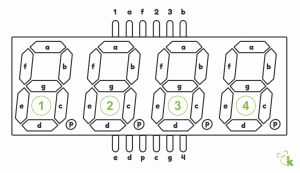
\includegraphics[width=0.5\linewidth]{imagenes/7_segmenos.png}
    \caption{Display de 7 segmentos 4 dígitos cátodo común}
    \label{fig:display}
\end{figure}


\subsection*{Modulo de Voz.}

El módulo ISD1820 es un grabador y reproductor de voz basado en el chip ISD1820. Su funcionamiento se centra en capturar, almacenar y reproducir mensajes de audio.

Utiliza un micrófono integrado para capturar el sonido. Al presionar el botón REC, el chip almacena la señal de audio de forma analógica en una memoria no volátil, donde la duración de la grabación es de aproximadamente 10 segundos.

Existen 2 modos para su reproducción.
PLAYE (Playback, Edge-activated): Al presionarlo una vez, reproduce el mensaje completo grabado.

PLAYL (Playback, Level-activated): Mientras se mantiene presionado, reproduce el mensaje de forma continua. Al soltarlo, la reproducción se detiene.

Control: Puede operarse manualmente con sus botones o de forma automática de forma externa enviando señlaes a sus pines de control (REC, PLAYE, PLAYL).

El chip incluye un amplificador de audio interno para manejar altavoces pequeños de aproximadamente 8 ohms y 0.5 Watts.

\begin{figure}[H]
    \centering
    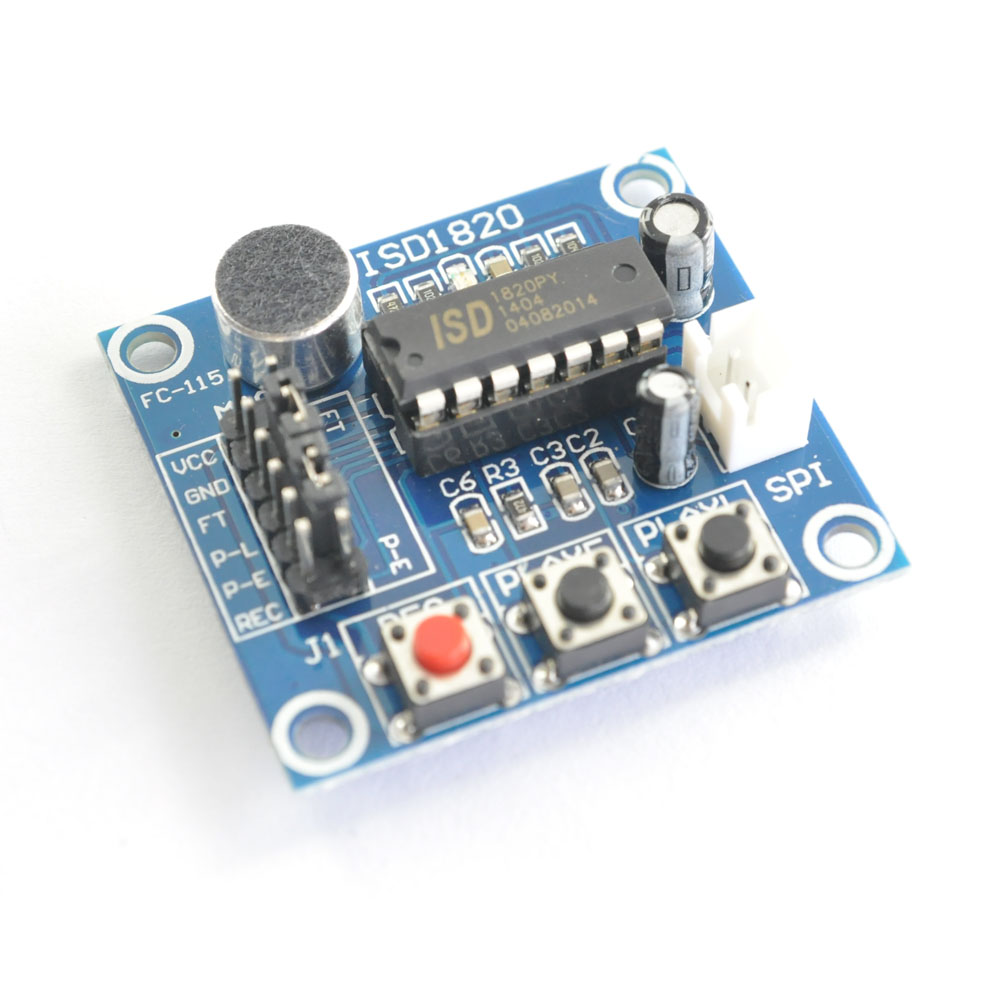
\includegraphics[width=0.5\linewidth]{imagenes/Modulo de voz.png}
    \caption{Modulo ISD1820}
    \label{fig:Voz}
\end{figure}

\subsection*{Comunicación RS232}

RS232 es una forma de comunicación en serie, lo que significa que la información se envía entre dispositivos un bit a la vez. Es una forma de comunicación asincrónica, lo que significa que los dispositivos de envío y recepción pueden operar en diferentes momentos.

El estándar RS232 define los detalles de cómo se envían y reciben los datos entre dispositivos. Las principales características del estándar RS232 son las siguientes:

Niveles de voltaje: La comunicación RS232 usa señales de voltaje para representar datos binarios. Un voltaje entre -3 V y -15 V representa un "1" binario (también conocido como "Marca"), mientras que un voltaje entre +3 V y +15 V representa un "0" binario (también conocido como "Espacio").
Transmisión de datos: RS232 admite comunicación dúplex completo, lo que significa que los datos se pueden enviar y recibir en ambas direcciones al mismo tiempo.
enmarcado: Cada paquete de datos enviado a través de RS232 contiene un bit de inicio, de 5 a 9 bits de datos, un bit de paridad opcional para la detección de errores y uno o dos bits de parada. Esta estructura se denomina "marco".
Tasa de baudios: La tasa de baudios es el número de cambios de señal por segundo que se envían o reciben a través de la línea. En RS232, la velocidad en baudios generalmente se especifica en bits por segundo (bps).
Líneas de control: RS232 utiliza varias líneas de control para gestionar el flujo de datos entre el transmisor y el receptor. Estos incluyen líneas como "Terminal de datos listo" (DTR), "Conjunto de datos listo" (DSR), "Solicitud de envío" (RTS) y "Listo para enviar" (CTS).
Comprobación de paridad: Este es un método para detectar errores en los datos transmitidos. La verificación de paridad agrega un bit adicional (el bit de paridad) a cada palabra de datos (generalmente un byte), que se establece para garantizar que el número total de 1 bits en la palabra (incluido el bit de paridad) sea siempre par o impar, según dependiendo de si se usa paridad par o impar.



\section{Desarrollo}
%! TEX root = C:\Users\osval\OneDrive - Instituto Politecnico Nacional\Codigos\Programacion\DLP\Practica_1\main.tex

\subsection*{Actividad 1. Funciones de Salida}

\textit{\textcolor{Verde}{Escritura, simulación e implementación de los códigos en VHDL y Verilog para programar las funciones de la tabla 1.1, repetida enseguida para su fácil implementación. Reportar diagrama de la entidad, códigos (VHDL, Verilog UCF), simulación y fotos editadas con texto explicativo. \\
Writing, simulation and implementation of the codes in VHDL and Verilog to program the functions of table 1.1, repeated immediately for easy implementation. Report codes, simulation and photographs.}}

\subsubsection*{Interpretación física de la tabla de verdad}

Para dar un significado práctico a la tabla de verdad mostrada, se propone un escenario de 
\textbf{sistema de control de riego en un invernadero}, donde las variables de entrada y 
salida corresponden a sensores y actuadores reales.

\textbf{Entradas (sensores)}
\begin{itemize}
    \item $A$: Sensor de humedad del suelo (1 = suelo seco, 0 = suelo húmedo).
    \item $B$: Sensor de radiación solar (1 = soleado, 0 = nublado).
    \item $C$: Sensor de nivel en tanque de agua (1 = tanque lleno, 0 = tanque vacío).
\end{itemize}

% ---------------------------------
% Lista de salidas (S4, S5, S6)
% ---------------------------------

\textbf{Salidas (actuadores/indicadores rediseñados)}

\begin{itemize}
    \item \textbf{S1: Indicador de Alerta / Modo de Acción (XOR)}\\
    \textbf{Expresión (SOP mínima):} \(\displaystyle S1 = \overline{A}\,\overline{B}\,C + \overline{A}\,B\,\overline{C} + A\,\overline{B}\,\overline{C} + ABC = A \oplus B \oplus C\).\\
    \textbf{Qué hace y cómo funciona:} S1 se enciende únicamente cuando un número \emph{impar} de sensores está activo (solo uno de ellos, o los tres a la vez). Funciona como un selector de modo lógico.\\
    - \emph{Razón física:} Indica que el sistema no está en un estado de reposo simple (como 000) ni en un estado de transición balanceado. Representa una condición que requiere una \emph{acción específica} o una \emph{alerta}, como cuando solo un sensor se activa (ej. solo el suelo está seco) o cuando todas las condiciones están al máximo (listo para regar bajo el sol).

    \item \textbf{S2: Indicador General de Actividad (OR)}\\
    \textbf{Expresión (SOP mínima):} \(\displaystyle S2 = A + B + C\).\\
    \textbf{Qué hace y cómo funciona:} S2 se enciende si \emph{cualquiera} de los sensores (A, B o C) está activo. Solo permanece apagado en el estado de reposo total (000).\\
    - \emph{Razón física:} Es el indicador más simple y fundamental del sistema. Sirve como una luz de "Sistema Ocupado" o "Condición Detectada", informando al operador que al menos una variable del invernadero no está en su estado base (húmedo, nublado y tanque vacío).

    \item \textbf{S3: Control de Ventilación por Coherencia Ambiental (XNOR)}\\
    \textbf{Expresión (SOP mínima):} \(\displaystyle S3 = \overline{A}\,\overline{B} + AB = A \odot B\).\\
    \textbf{Qué hace y cómo funciona:} S3 activa un actuador cuando las condiciones de humedad del suelo (A) y sol (B) son \emph{coherentes}; es decir, ambas están inactivas (húmedo y nublado) o ambas están activas (seco y soleado).\\
    - \emph{Razón física:} Es ideal para manejar la ventilación. Si está húmedo y nublado ($A=0, B=0$), las compuertas se cierran para conservar calor. Si está seco y soleado ($A=1, B=1$), las compuertas se abren para disipar el calor y prepararse para el riego. Si las condiciones son mixtas, la ventilación permanece en un estado neutro.
    \item \textbf{S4: Ventilador de Circulación}\\
    \textbf{Expresión (SOP mínima):} \(\displaystyle S4 = \overline{A}BC + AB\overline{C} = B \cdot (A \oplus C)\).\\
    \textbf{Qué hace y cómo funciona:} S4 enciende el ventilador únicamente cuando está \emph{soleado} ($B=1$) y las condiciones de agua presentan un contraste: suelo húmedo y tanque lleno ($A=0, C=1$) o suelo seco y tanque vacío ($A=1, C=0$).\\
    - \emph{Razón física:} Actúa para regular la temperatura y humedad en momentos de alta radiación solar. Si hay agua y humedad, previene la condensación. Si no hay agua y el suelo está seco, intenta mitigar el estrés térmico en las plantas.

    \item \textbf{S5: Sistema de Calefacción/Luz Artificial}\\
    \textbf{Expresión (SOP mínima):} \(\displaystyle S5 = \overline{A}\,\overline{B}\,\overline{C}\).\\
    \textbf{Qué hace y cómo funciona:} S5 activa un sistema de soporte (calefactor o luz de crecimiento) solo en el escenario más pasivo y frío: \emph{suelo húmedo} ($A=0$), \emph{nublado} ($B=0$) y \emph{tanque vacío} ($C=0$).\\
    - \emph{Razón física:} Compensa la falta de energía (sol) y el riesgo de bajas temperaturas en la condición de inactividad total, protegiendo a las plantas de un ambiente adverso y manteniendo un microclima estable.

    \item \textbf{S6: Alarma Crítica por Falta de Agua}\\
    \textbf{Expresión (SOP mínima):} \(\displaystyle S6 = A \cdot \overline{C}\).\\
    \textbf{Qué hace y cómo funciona:} S6 dispara una alarma sonora o visual únicamente si el suelo está \emph{seco} ($A=1$) \textbf{y}, al mismo tiempo, el tanque está \emph{vacío} ($C=0$).\\
    - \emph{Razón física:} Señaliza la condición más peligrosa para el cultivo. El sistema no puede actuar (regar) y necesita intervención humana inmediata para rellenar el tanque y evitar la pérdida de las plantas.
\end{itemize}

% ---------------------------------------
% Lista completa de casos (000 -- 111)
% ---------------------------------------

\textbf{Interpretación de casos}

\begin{enumerate}
    \item \textbf{Caso 000: Suelo húmedo, sin sol, tanque vacío.}\\
    - Entradas: $A=0$, $B=0$, $C=0$.\\
    - Interpretación: Escenario de inactividad total. Ambiente frío, oscuro y sin recursos hídricos.\\
    - Salidas: 
        \begin{itemize}
            \item S3=1 (compuerta en modo conservación, ej. cerrada). 
            \item S5=1 (sistema de calefacción activo para proteger del frío). 
        \end{itemize}
    - \emph{Razón:} El sistema entra en modo de protección pasiva, conservando calor y aportando energía artificialmente.

    \item \textbf{Caso 001: Suelo húmedo, sin sol, tanque lleno.}\\
    - Entradas: $A=0$, $B=0$, $C=1$.\\
    - Interpretación: Condiciones estables y con agua disponible. No se requiere acción de riego o ventilación.\\
    - Salidas: 
        \begin{itemize}
            \item S1=1 (alerta de estado, hay un sensor activo). 
            \item S2=1 (indicador general activo).
            \item S3=1 (compuerta en modo conservación).
        \end{itemize}
    - \emph{Razón:} El sistema está en espera, monitorizando una condición normal y con recursos.

    \item \textbf{Caso 010: Suelo húmedo, con sol, tanque vacío.}\\
    - Entradas: $A=0$, $B=1$, $C=0$.\\
    - Interpretación: Día soleado, el suelo aún no necesita agua, pero no hay reservas.\\
    - Salidas:
        \begin{itemize}
            \item S1=1 (alerta de estado).
            \item S2=1 (indicador general activo).
        \end{itemize}
    - \emph{Razón:} El sistema se mantiene en alerta por la combinación de sol (demanda de evaporación) y tanque vacío (sin capacidad de respuesta).

    \item \textbf{Caso 011: Suelo húmedo, con sol, tanque lleno.}\\
    - Entradas: $A=0$, $B=1$, $C=1$.\\
    - Interpretación: Condición ideal. Hay sol, el suelo está húmedo y hay agua de reserva.\\
    - Salidas:
        \begin{itemize}
            \item S2=1 (indicador general activo).
            \item S4=1 (ventilador activo para circular aire y controlar la temperatura/humedad).
        \end{itemize}
    - \emph{Razón:} Se realiza una gestión proactiva del clima para mantener las condiciones óptimas.

    \item \textbf{Caso 100: Suelo seco, sin sol, tanque vacío.}\\
    - Entradas: $A=1$, $B=0$, $C=0$.\\
    - Interpretación: ¡Problema! El suelo necesita agua, pero no hay ni sol ni agua en el tanque.\\
    - Salidas:
        \begin{itemize}
            \item S1=1 (alerta de estado).
            \item S2=1 (indicador general activo).
            \item S6=1 (alarma crítica por falta de agua).
        \end{itemize}
    - \emph{Razón:} El sistema no puede solucionar el problema y escala la situación a una alarma para el operario.

    \item \textbf{Caso 101: Suelo seco, sin sol, tanque lleno.}\\
    - Entradas: $A=1$, $B=0$, $C=1$.\\
    - Interpretación: Se necesita regar y hay agua disponible, aunque esté nublado.\\
    - Salidas:
        \begin{itemize}
            \item S2=1 (indicador general activo).
        \end{itemize}
    - \emph{Razón:} Sistema en espera para activar el riego (que sería una función lógica de $A \cdot C$).

    \item \textbf{Caso 110: Suelo seco, con sol, tanque vacío.}\\
    - Entradas: $A=1$, $B=1$, $C=0$.\\
    - Interpretación: ¡Emergencia! El suelo está seco, el sol acelera la deshidratación y no hay agua.\\
    - Salidas:
        \begin{itemize}
            \item S2=1 (indicador general activo).
            \item S3=1 (compuerta en modo coherencia, ej. abierta para ventilar).
            \item S4=1 (ventilador activo para intentar reducir el estrés por calor).
            \item S6=1 (alarma crítica activa, es la máxima prioridad).
        \end{itemize}
    - \emph{Razón:} El sistema activa todas las medidas paliativas posibles (ventilación) mientras alerta de la condición crítica.

    \item \textbf{Caso 111: Suelo seco, con sol, tanque lleno.}\\
    - Entradas: $A=1$, $B=1$, $C=1$.\\
    - Interpretación: Momento clave para el riego. El suelo lo necesita y las condiciones son de alta demanda energética.\\
    - Salidas:
        \begin{itemize}
            \item S1=1, S2=1, S3=1 (todos los indicadores y la ventilación están activos).
        \end{itemize}
    - \emph{Razón:} El sistema está en su estado de máxima actividad, listo para desplegar todas sus funciones (riego, ventilación, etc.).
\end{enumerate}

% =============================
% TABLA DE VERDAD
% =============================
\textbf{Tabla de verdad}

\begin{table}[h!]
\centering
\caption{Tabla de verdad completa del sistema de control}
\begin{tabular}{|c|c|c||c|c|c||c|c|c|}
\hline
\multicolumn{3}{|c||}{\textbf{Entradas}} & \multicolumn{6}{c|}{\textbf{Salidas}} \\
\hline
\textbf{A} & \textbf{B} & \textbf{C} & \textbf{S1} & \textbf{S2} & \textbf{S3} & \textbf{S4} & \textbf{S5} & \textbf{S6} \\
\hline \hline
0 & 0 & 0 & 0 & 0 & 1 & \textbf{0} & \textbf{1} & \textbf{0} \\
\hline
0 & 0 & 1 & 1 & 1 & 1 & \textbf{0} & \textbf{0} & \textbf{0} \\
\hline
0 & 1 & 0 & 1 & 1 & 0 & \textbf{0} & \textbf{0} & \textbf{0} \\
\hline
0 & 1 & 1 & 0 & 1 & 0 & \textbf{1} & \textbf{0} & \textbf{0} \\
\hline
1 & 0 & 0 & 1 & 1 & 0 & \textbf{0} & \textbf{0} & \textbf{1} \\
\hline
1 & 0 & 1 & 0 & 1 & 0 & \textbf{0} & \textbf{0} & \textbf{0} \\
\hline
1 & 1 & 0 & 0 & 1 & 1 & \textbf{1} & \textbf{0} & \textbf{1} \\
\hline
1 & 1 & 1 & 1 & 1 & 1 & \textbf{0} & \textbf{0} & \textbf{0} \\
\hline
\end{tabular}
\end{table}


\subsubsection*{Código VHDL}

\lstinputlisting[
  language=VHDL, 
  caption={Código completo para el sistema de tres entradas y 6 salidas con interpretación física.},
  label={lst:sumador_vhd}
]{Codigos/Ejercicio1_VH.vhd}

\subsubsection*{Código Verilog}

\lstinputlisting[
  language=Verilog,
  caption={Código completo para el sistema de tres entradas y 6 salidas con interpretación física.},
  label={lst:tb_verilog}
]{Codigos/Ejercicio1.v}

\subsubsection*{Simulación}

Por la configuración en Pull-Up de los switches en la tarjeta de desarrollo en la simulación se visualizan los valores de la tabla invertidos, ejemplo cuando la entrada es 111, la simulación muestra los valores a la salida de un 000.

\begin{figure}
    \centering
    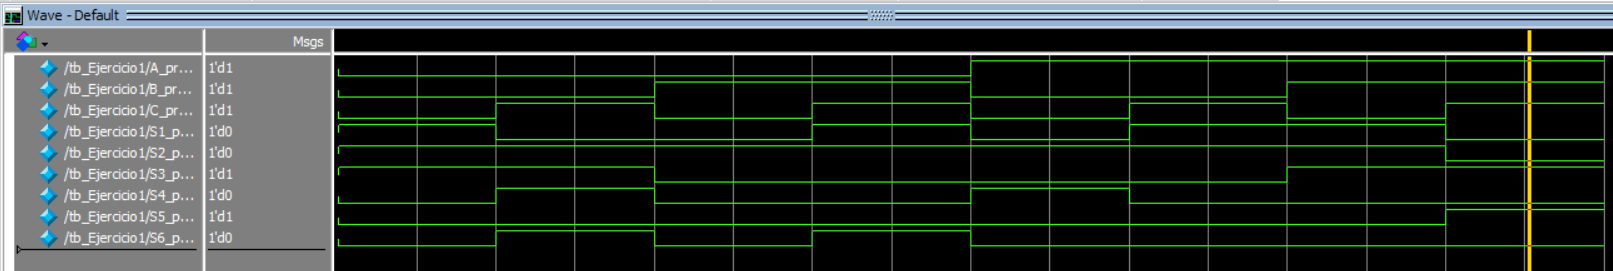
\includegraphics[width=1\linewidth]{imagenes/Sim_1.png}
    \caption{Simulación 1 en Questa}
    \label{fig:Sim_1}
\end{figure}

\subsubsection*{Fotos}

\begin{figure}[H]
    \centering
    % Primera imagen
    \begin{subfigure}{0.45\linewidth}
        \centering
        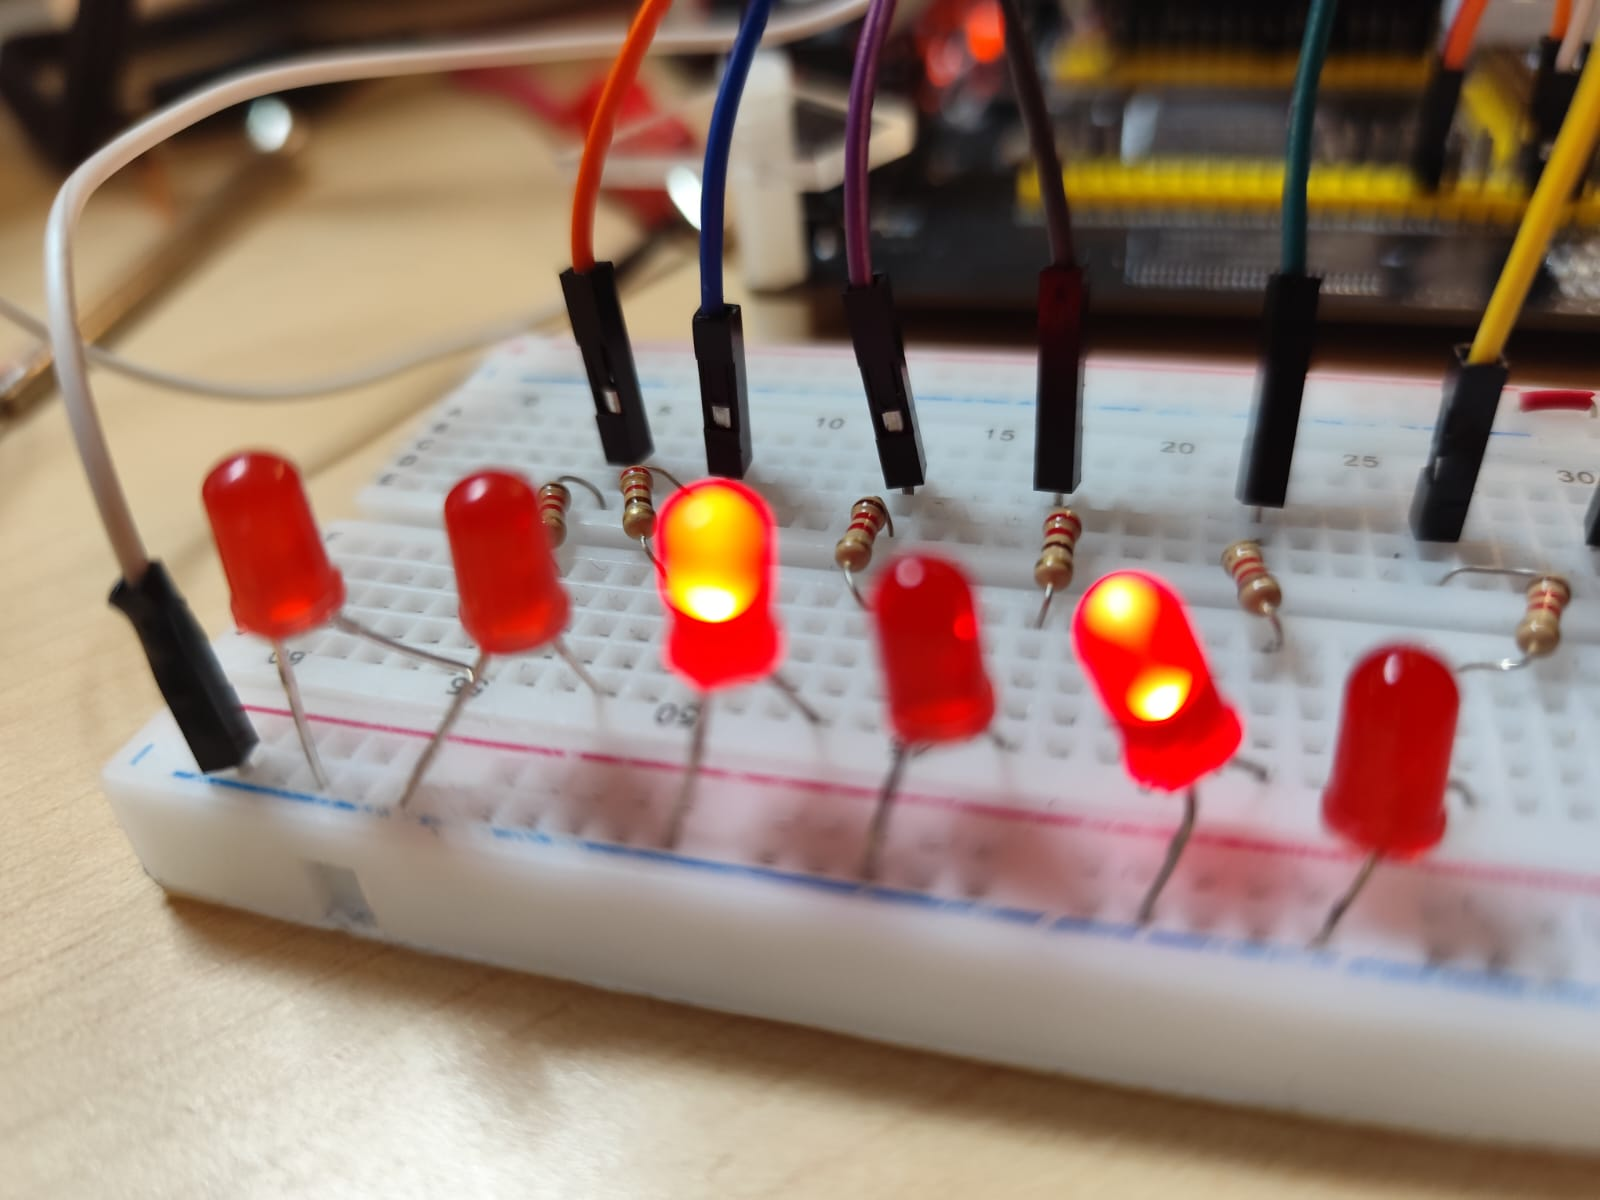
\includegraphics[width=\linewidth]{imagenes/000.png}
        \caption{Leds de prueba con entrada 000}
        \label{fig:000}
    \end{subfigure}
    \hfill
    % Segunda imagen
    \begin{subfigure}{0.45\linewidth}
        \centering
        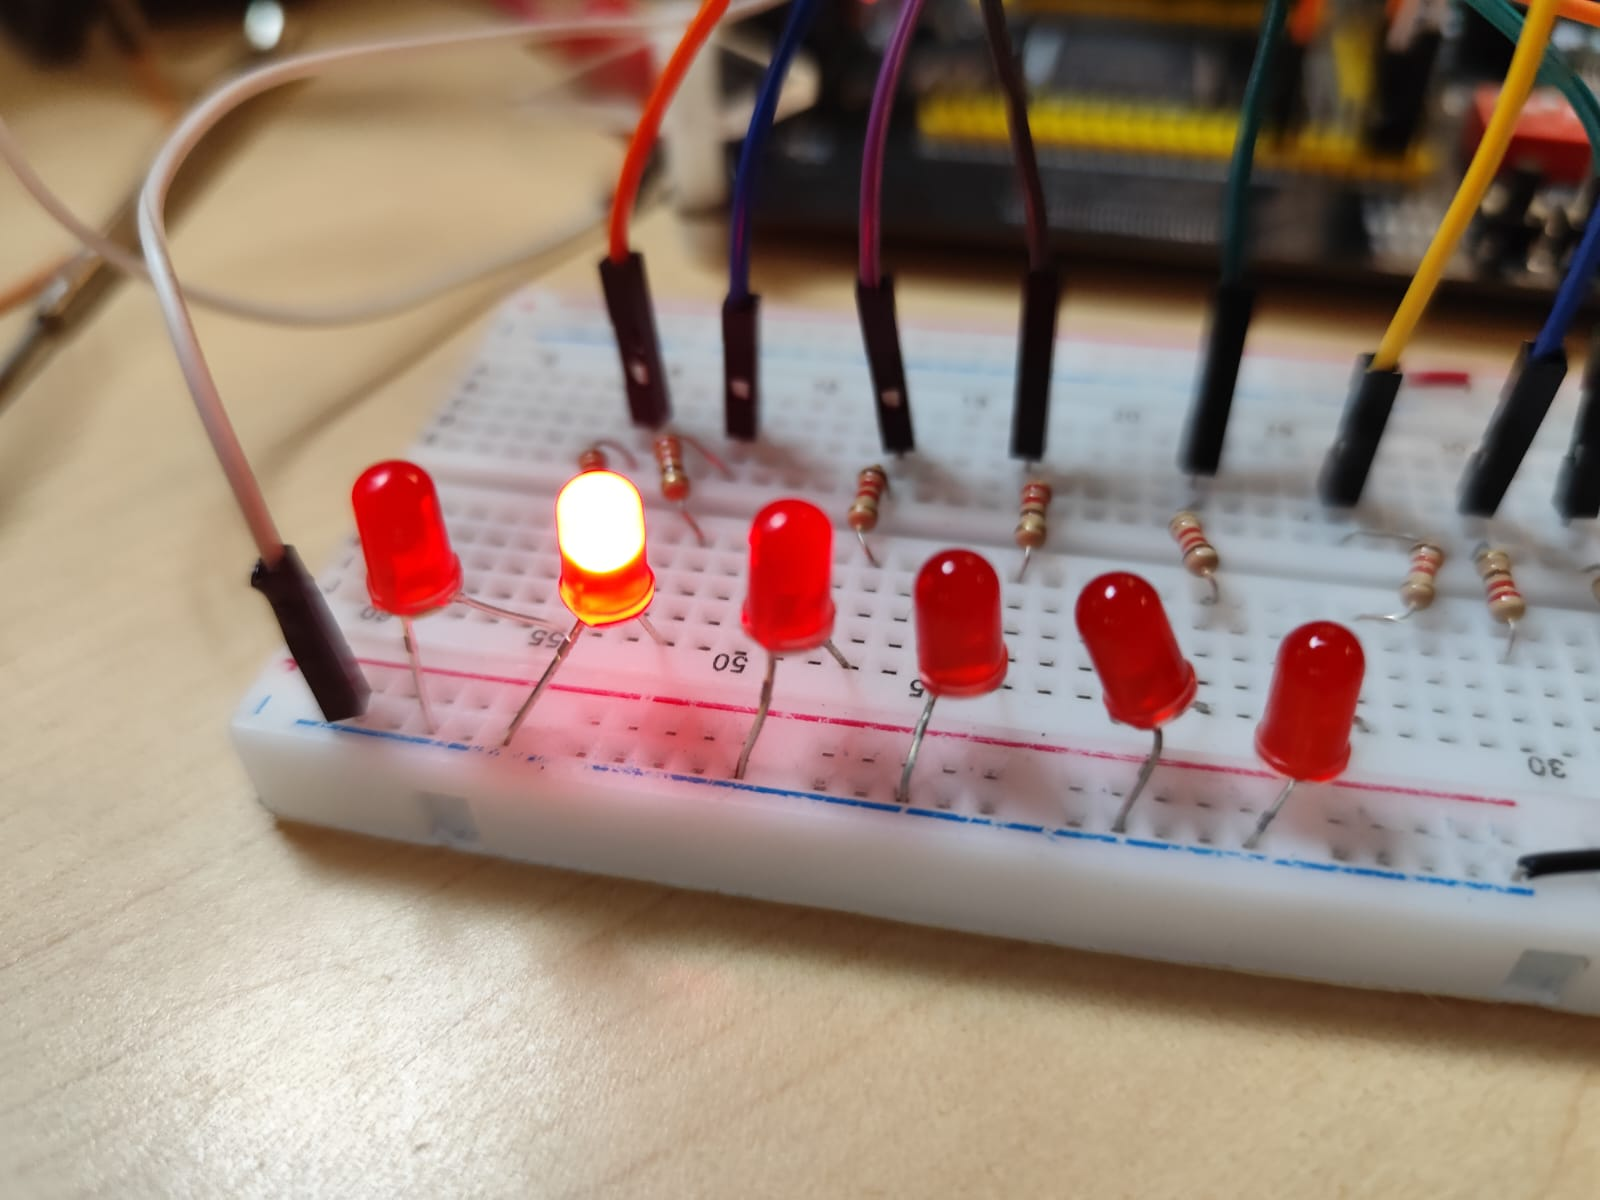
\includegraphics[width=\linewidth]{imagenes/101.png}
        \caption{Leds de prueba con entrada 101}
        \label{fig:101}
    \end{subfigure}
    % Pie de figura general
    \caption{Pruebas de los leds con distintas entradas}
    \label{fig:leds}
\end{figure}


\subsection*{Actividad 2. Registro 8 bits}

\textit{\textcolor{Verde}{Escritura, simulación e implementación de los códigos en VHDL y Verilog para programar un registro de 8 bits basado en el FF-D. Reportar códigos, simulación y fotos. \\
Writing, simulation, and implementation of the codes in VHDL and Verilog to program a 4-bit register based on the FF-D. Report codes, simulation and photographs.}}

En este puntos se realizo un registro de 8 bits donde tenemos 8 entradas y 8 salidas físicas para poder visualizar que los datos del registro se guarden correctamente al presionar un push button. Notemos que el retardo de dos ciclos se debe a que tu circuito realiza dos tareas de verificación antes de guardar los datos, cada una tomando un ciclo de reloj:

Ciclo 1: Sincronizar. El sistema primero "sincroniza" la señal del botón con el reloj interno para evitar errores. Es el primer paso para "escuchar" limpiamente tu pulsación.

Ciclo 2: Detectar el Borde. Luego, el circuito compara el estado actual del botón (presionado) con el anterior (no presionado) para confirmar que es una acción nueva. Al detectar este cambio, genera el pulso\_captura que dura exactamente un ciclo.

Solo después de estos dos pasos de preparación, el pulso\_captura le da la orden a los LEDs para que capturen el valor.

\subsubsection*{Codigo VHDL}

\lstinputlisting[
  language=VHDL, 
  caption={Código completo para el registro de 8 Bits},
  label={lst:sumador_vhd}
]{Codigos/Ejercicio2_VH.vhd}

\subsubsection*{Verilog}

\lstinputlisting[
  language=Verilog,
  caption={Código completo para el registro de 8 Bits.},
  label={lst:tb_verilog}
]{Codigos/Ejercicio2.v}

\subsubsection*{Simulación}

El retardo de dos ciclos se debe a que tu circuito realiza dos tareas de verificación antes de guardar los datos, cada una tomando un ciclo de reloj:

Ciclo 1: Sincronizar. El sistema primero "sincroniza" la señal del botón con el reloj interno para evitar errores. Es el primer paso para "escuchar" limpiamente tu pulsación.

Ciclo 2: Detectar el Borde. Luego, el circuito compara el estado actual del botón (presionado) con el anterior (no presionado) para confirmar que es una acción nueva. Al detectar este cambio, genera el pulso\_captura que dura exactamente un ciclo.

Solo después de estos dos pasos de preparación, el pulso\_captura le da la orden a los LEDs para que capturen el valor.

\begin{figure}
    \centering
    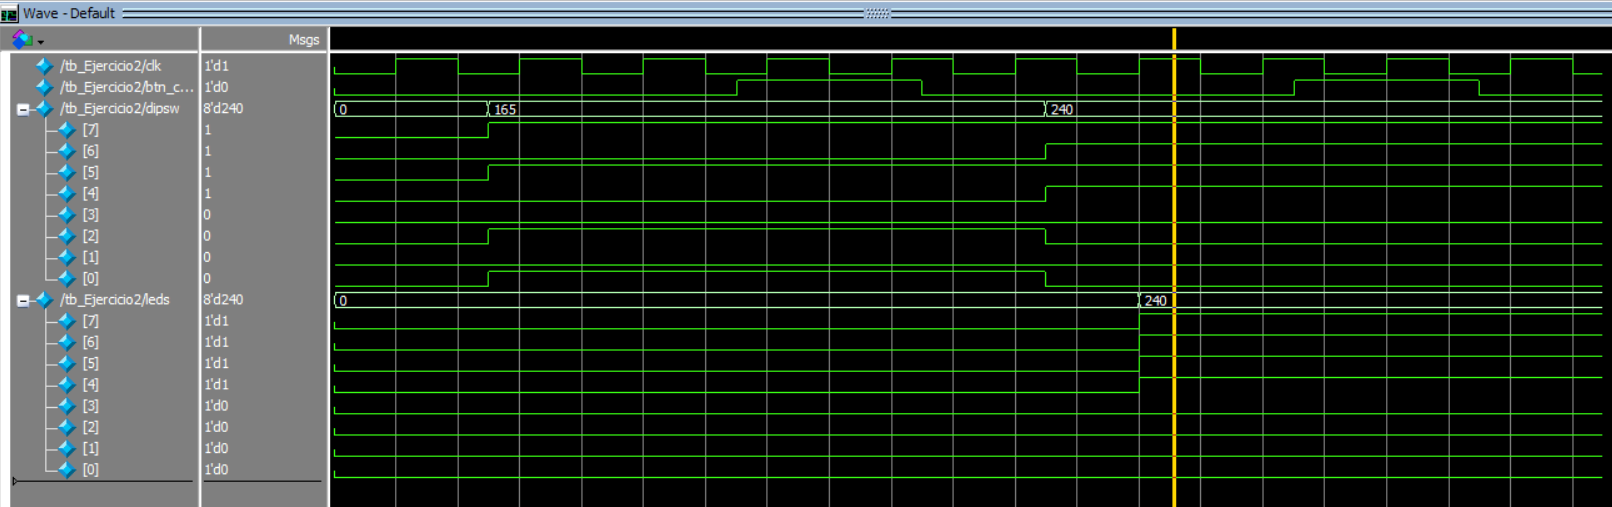
\includegraphics[width=1\linewidth]{imagenes/Sim_2.png}
    \caption{Simulación 2 en Questa}\label{fig:Sim_2}
\end{figure}

\subsubsection*{Fotos}

\begin{figure}[H]
    \centering
    % Primera imagen
    \begin{subfigure}{0.45\linewidth}
        \centering
        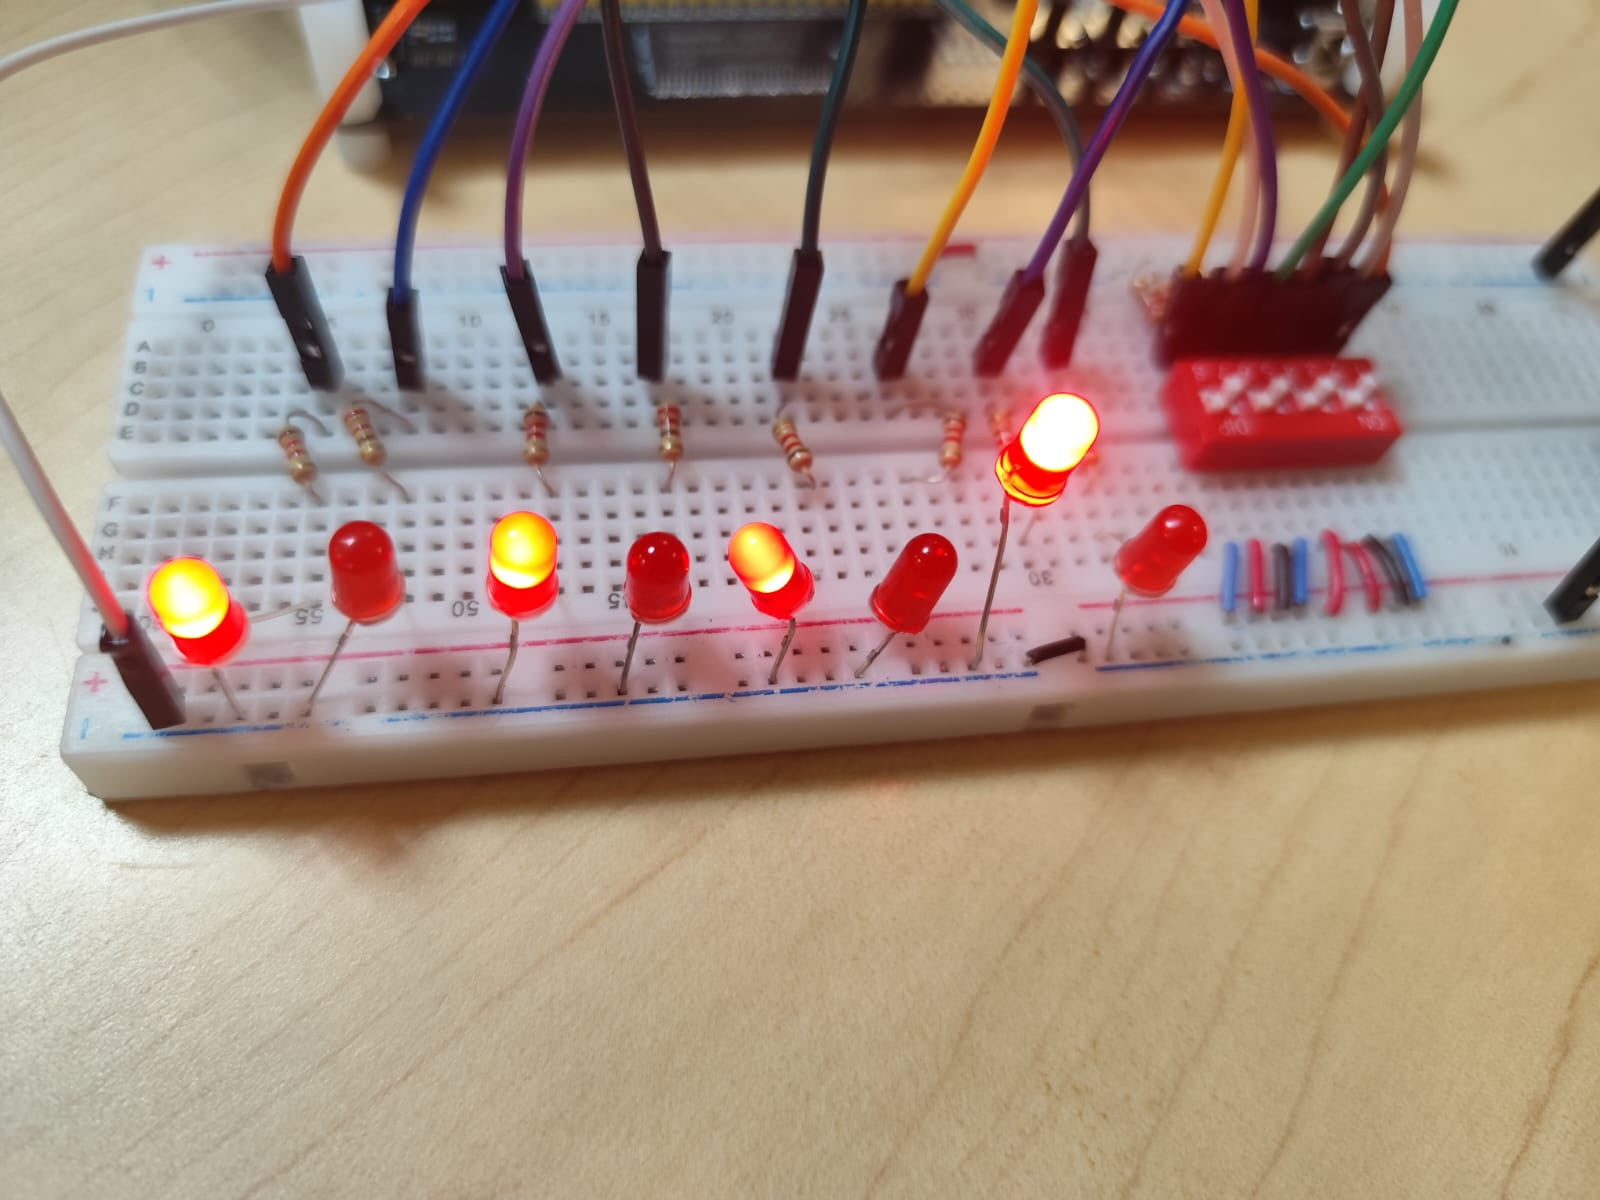
\includegraphics[width=\linewidth]{imagenes/Registro1.png}
        \caption{Registro 1}\label{fig:R1}
    \end{subfigure}
    \hfill
    % Segunda imagen
    \begin{subfigure}{0.45\linewidth}
        \centering
        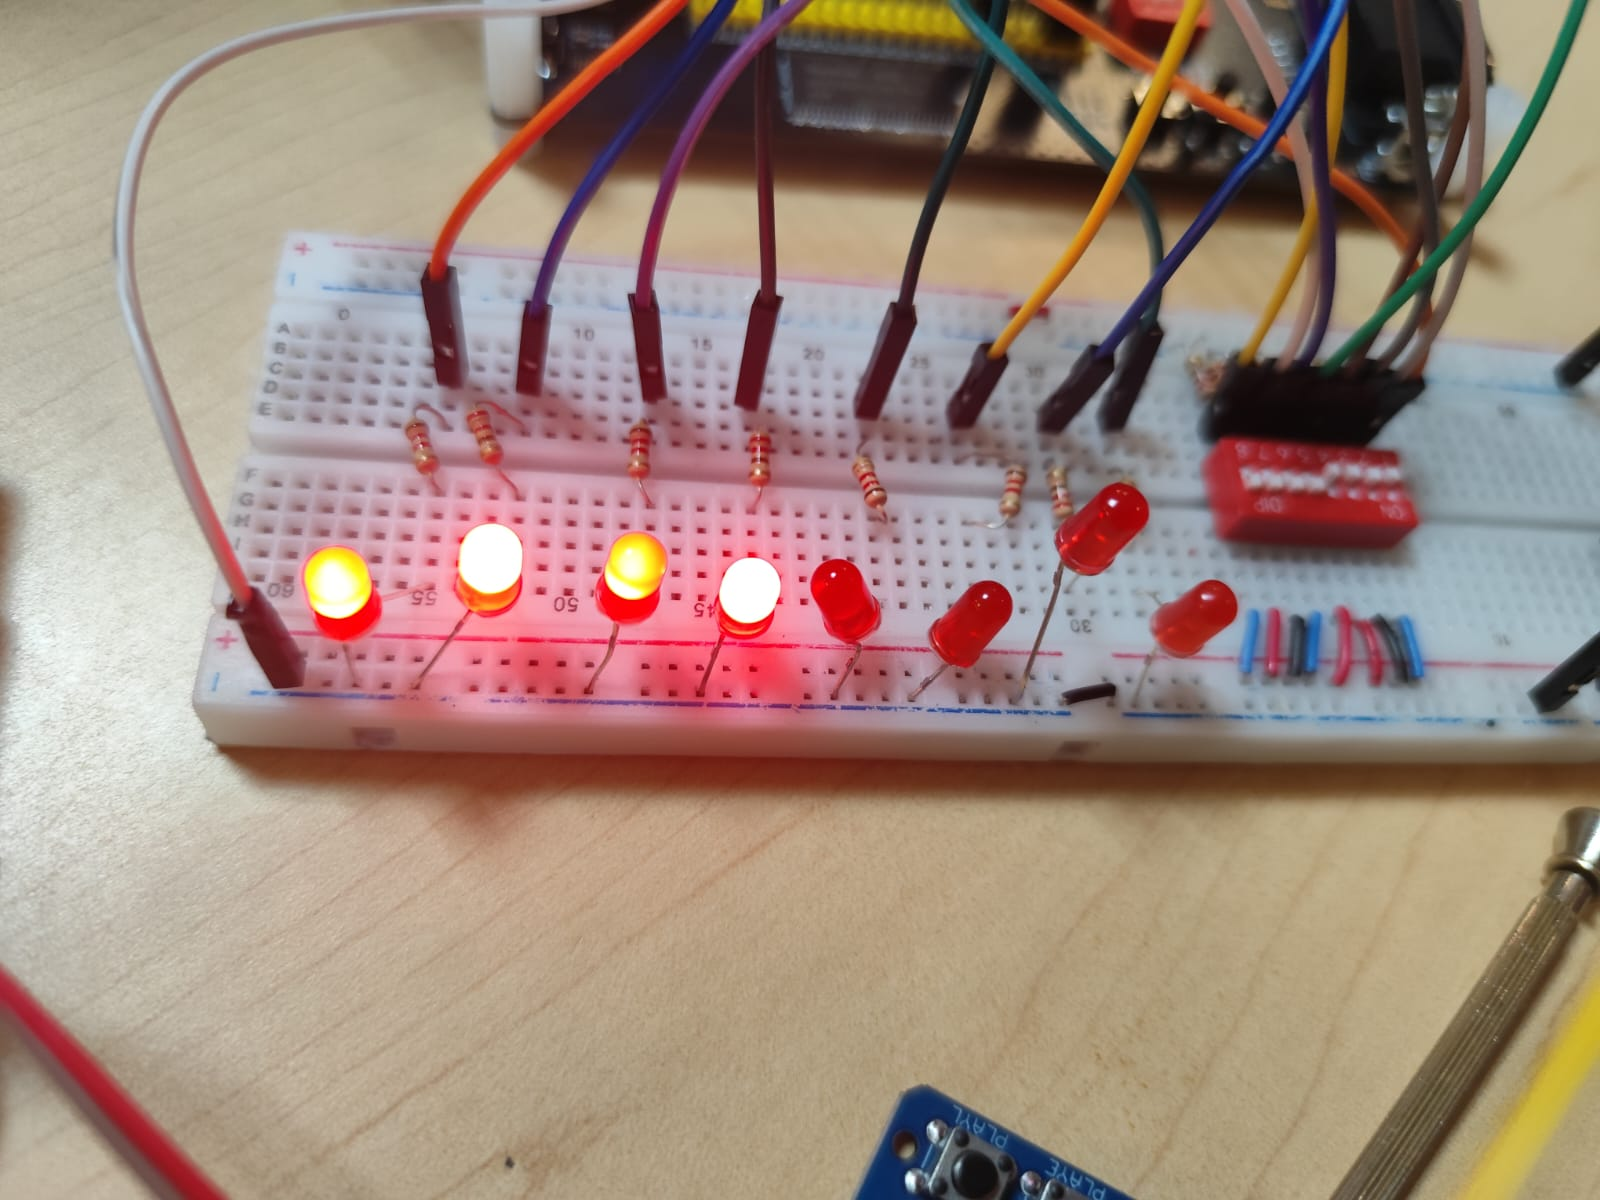
\includegraphics[width=\linewidth]{imagenes/Registro2.png}
        \caption{Registro 2}\label{fig:R2}
    \end{subfigure}
    % Pie de figura general
    \caption{Pruebas de los leds para registro de 8 bits}\label{fig:leds2}
\end{figure}

\subsection*{Actividad 3. Contador de 4 bits}

\textit{\textcolor{Verde}{Escritura, simulación e implementación de los códigos en VHDL y Verilog para programar un contador binario de 4 bits ascendente-descendente ciclado, con interruptor de dirección (1 cuenta ascendente, 0 cuenta descendente), botón de reset en bajo y un botón de habilitación (inicio), con salida a display de 7 segmentos (0--9, A--F). Reportar códigos, simulación y fotos. \\
Writing, simulation, and implementation of the codes in VHDL and Verilog to program a cycled up-down binary 4-bit counter with address switch (1 up count, 0 counts down), reset button on bass and an enable button (start) with 7 seg display (0--9, A--F). Report codes, simulations, and photographs.}}

Para este punto se realizo un contador de 4 bits que muestra los datos de conteo en un display de 7 segmentos del 0 al 9 y de A-F de forma ascendente y descendente, al igual que cuenta con un switch para detener el conteo, un switch para cambiar la direccion de conteo y un push button para reiniciar el conteo. 

\subsubsection*{Codigo VHDL}

\lstinputlisting[
  language=VHDL, 
  caption={Código completo para el contador de 4 Bits.},
  label={lst:sumador_vhd}
]{Codigos/p3.vhd}

\subsubsection*{Verilog}

\lstinputlisting[
  language=Verilog,
  caption={Código completo para el contador de 4 Bits.},
  label={lst:tb_verilog}
]{Codigos/Ejercicio3_Veri.v}

\subsubsection*{Simulación}


\begin{figure}
    \centering
    \includegraphics[width=1\linewidth]{imagenes/Sim_3.png}
    \caption{Simulacion 3 en Questa}\label{fig:Sim_3}
\end{figure}

\subsubsection*{Fotos}

\begin{figure}[H]
    \centering
    % Primera imagen
    \begin{subfigure}{0.45\linewidth}
        \centering
        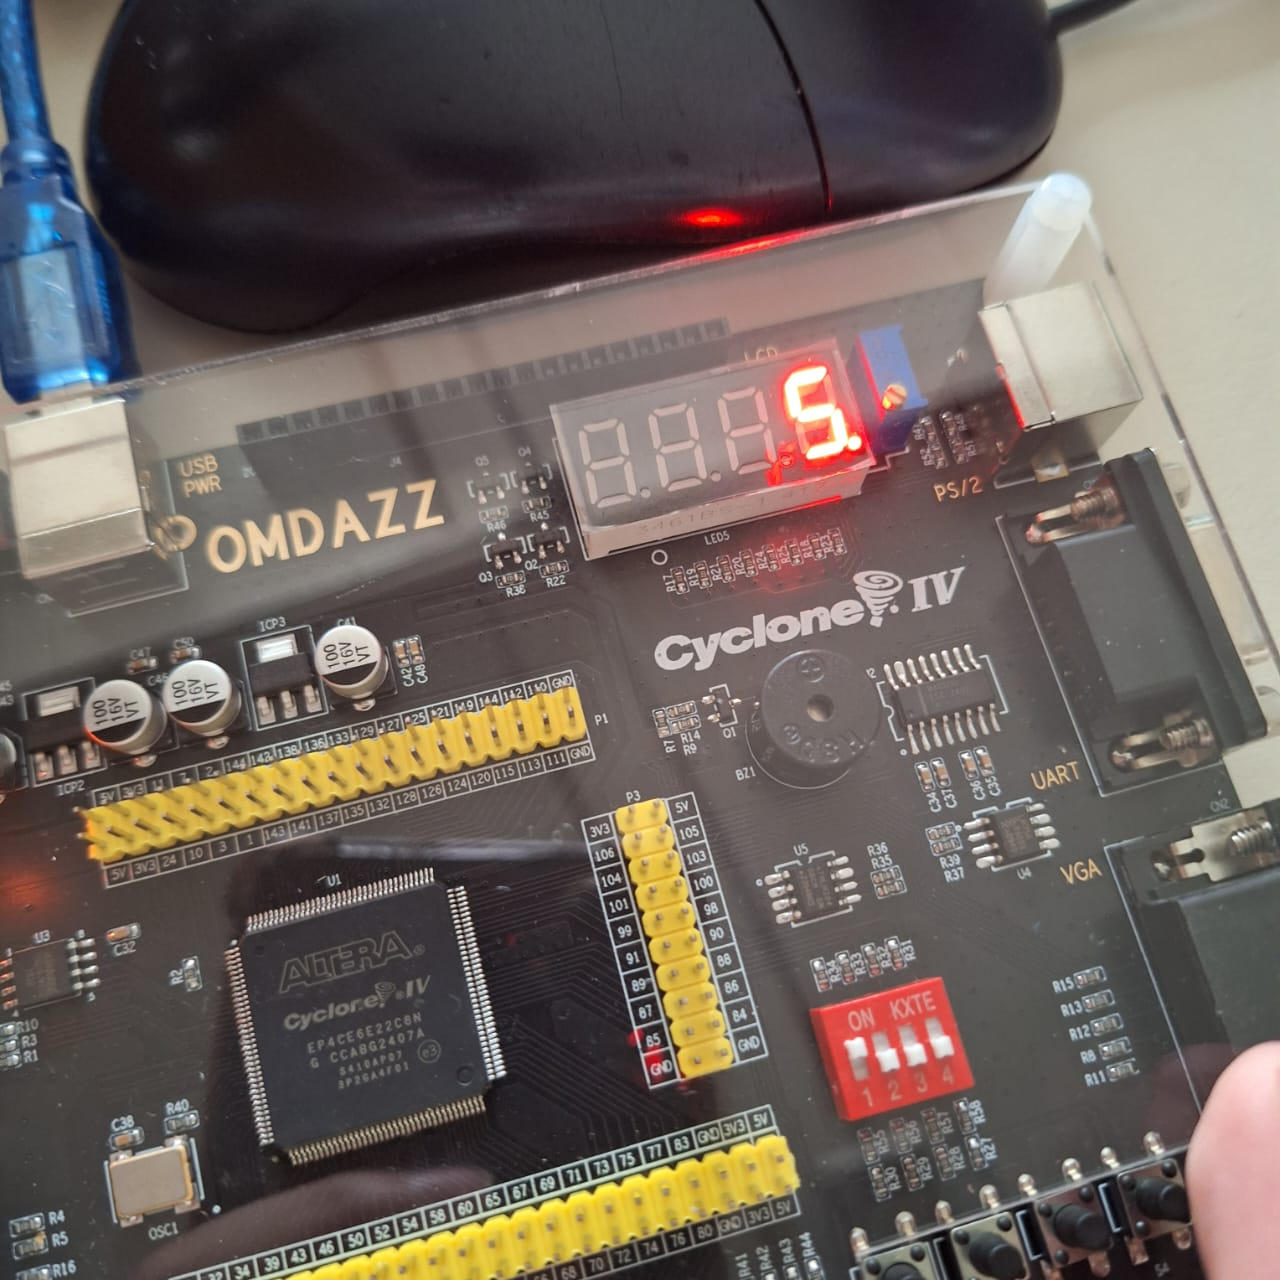
\includegraphics[width=\linewidth]{imagenes/Cnt8.jpg}
        \caption{Contador 4 Bits ascendente.}\label{fig:R1-1}
    \end{subfigure}
    \hfill
    % Segunda imagen
    \begin{subfigure}{0.45\linewidth}
        \centering
        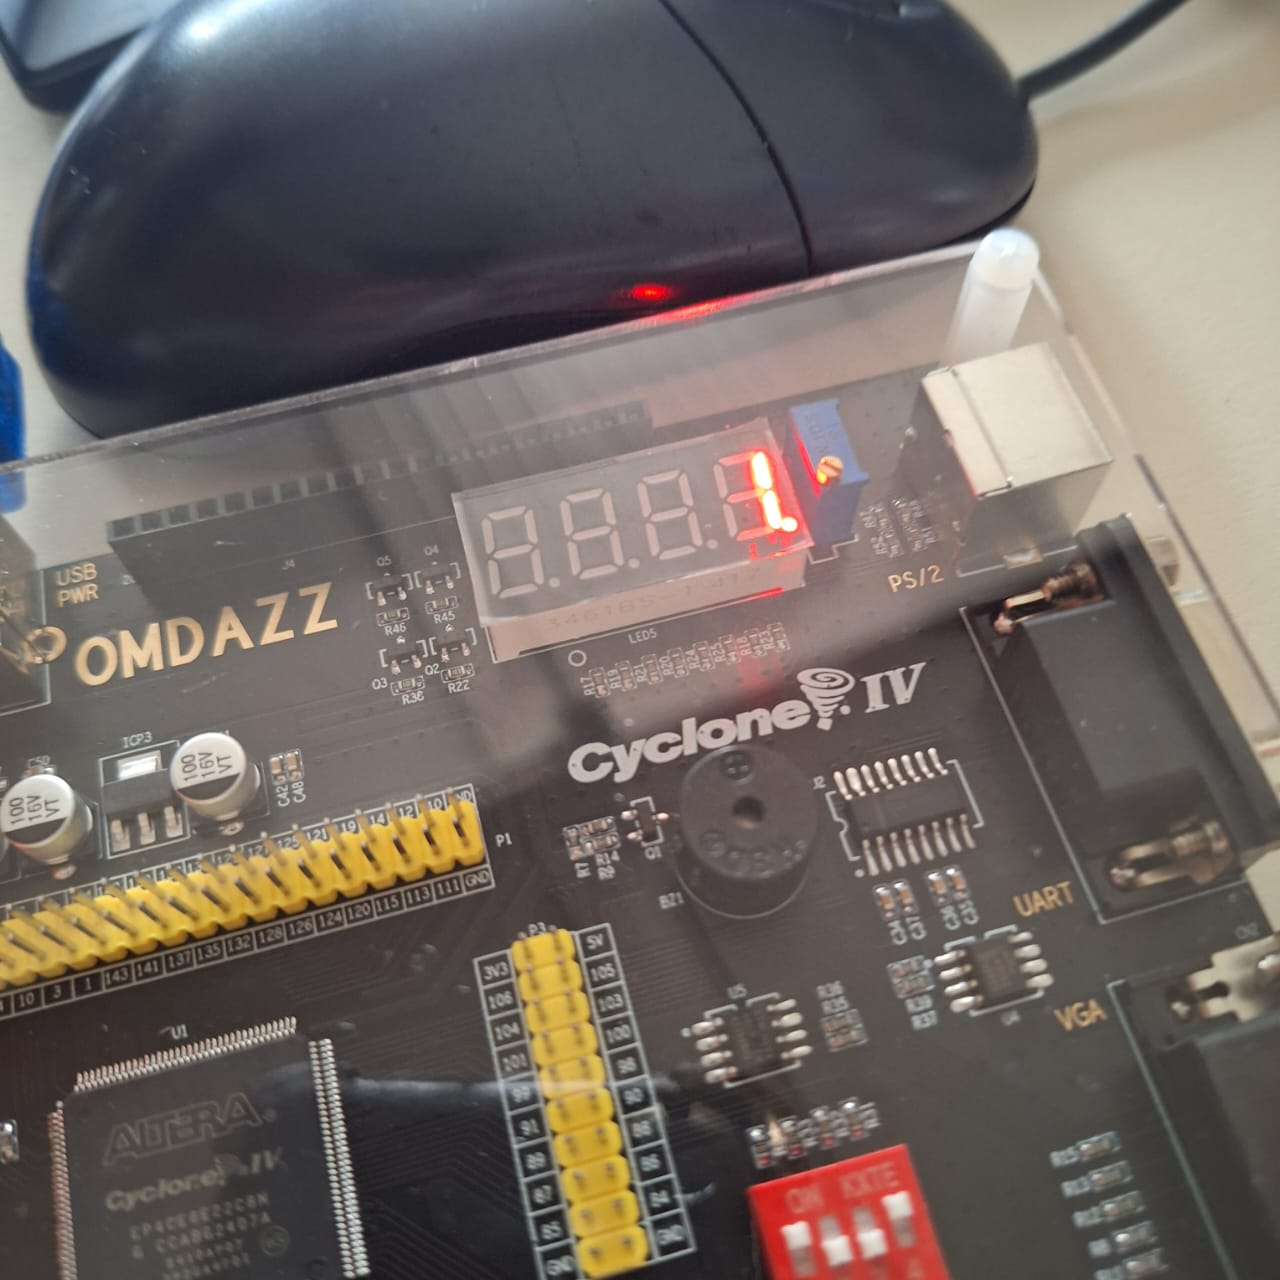
\includegraphics[width=\linewidth]{imagenes/Cnt8_2.jpg}
        \caption{Contador 4 Bits descendente.}\label{fig:R2-2}
    \end{subfigure}
    % Pie de figura general
    \caption{Implementación física en un display de 7 segmentos incorporado en la tarjeta de desarrollo.}\label{fig:leds3}
\end{figure}

\subsection*{Actividad 4. Sirenas}

\textit{\textcolor{Verde}{Implementar un circuito para tocar la sirena (a) de policía y (b) de una ambulancia con
distintos barridos de tonos, controlando en encendido y apagado con un interruptor
(SW0). Recuerde que la salida se conecta a una bocina con su etapa de potencia de audio.
Reportar códigos, fotos y videos.\\
Implement a circuit to play the siren of (i) police and (ii) an ambulance with different
sweeps of tones, controlling then on and off with a switch (SW0). Connect the output to
a speaker with audio stage power. Report code, phtos and video.}}

Para el punto 4 se desarrollaron una sirena de policia y una sirena de ambulancia usando un buzzer incluido en la tarjeta de desarrollo y un switch para hacer el cambio entre sirenas.

\subsubsection*{Código VHDL}

\lstinputlisting[
  language=VHDL, 
  caption={Código completo para el sistema de alarma para una patrulla de policia y una ambulancia.},
  label={lst:sumador_vhd}
]{Codigos/Ejercicio4_VH.vhd}

\subsubsection*{Verilog}

\lstinputlisting[
  language=Verilog,
  caption={Código completo para el sistema de alarma para una patrulla de policía y una ambulancia.},
  label={lst:tb_verilog}
]{Codigos/Ejercicio4.v}

\subsubsection*{Simulación}

\begin{figure}
    \centering
    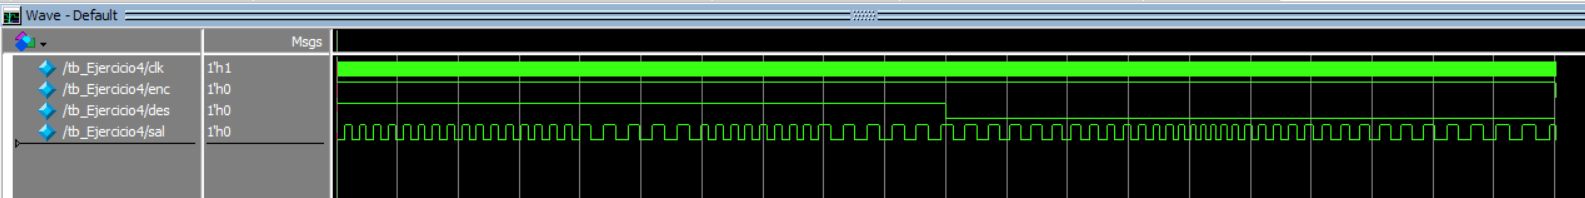
\includegraphics[width=1\linewidth]{imagenes/Sim_4.png}
    \caption{Simulación 4 en Questa}\label{fig:Sim_4}
\end{figure}


\subsubsection*{Fotos}

Al ser una actividad auditiva no agregamos fotografía de la implementación, en su lugar adjuntamos un video en la asignación de Classroom junto con este pdf.

\subsection*{Actividad 5. Modulo de Voz}

\textit{\textcolor{Verde}{Implementar el diseño de dos circuitos utilizando alto nivel (Top Level Design, figura
1.16), uno con VHDL y uno con Verilog. Dentro de cada diseño activar un mensaje de
audio utilizando un módulo reproductor comercial (ver figura 1.17), con una bocina de
4--8 /Omega y 3--4 W con su etapa de potencia de audio. Reportar códigos y fotos. Nota: deben
se distintos a los otros puntos entregados.\\
Implement the design of two circuits using high level (Top Level Design, figure 1.16),
one with VHDL and one with Verilog. In each design activate a voice message using a
commercial module (see figure 1.17) and 4--8~$\Omega$, 2--3~W speaker with audio power output.
Report codes and photos. Note: must be different to another point reviewed.}}


\subsubsection*{Codigo Verilog}

\lstinputlisting[
  language=Verilog,
  caption={Código en para grabación y reproducción de audio.},
  label={lst:Voz_verilog}
]{Codigos/Ejercicio6.v}




\subsection*{Actividad 6. Encoder y protocolo RS232}

\textit{\textcolor{Verde}{Implementar con TLD un circuito de prueba del giro de un encoder mecánico rotatorio
(ver figura 1.18), mostrado en las referencias, uno para el PmodALS, o el del módulo
RS232 con una separación de por lo menos 1m (ver figuras 1.19 y 1.20), mostrado en
el documento (PDLP 05 RS232.pdf), u otro módulo externo similar. Reportar códigos
y fotos.\\
Implement using TLD a test circuit for rotatory mechanical encoder (see figure 1.18),
showing in references, one for the PmodALS, or RS232 module with at least 1m between
the boards (see figures 1.19 and 1.20) o showed in the document (PDLP 05 RS232.pdf)
or another similar external module. Report codes and photos.}}


En el punto 6 realizamos un Top Level Designed para realizar la comunicación entre una CPLD con un chip MAX II, y una tarjeta de desarrollo cyclone 4, por medio del protocolo de comunicación RS232, haciendo que la cyclone 4 lea los datos del encoder mecánico y mande los datos por el protocolo de comunicación hacia la CPLD y esta la muestre visualmente por medio de LEDS.\ 

\subsubsection*{Códigos VHDL}

\lstinputlisting[
  language=VHDL, 
  caption={Código TLD.},
  label={TLD}
]{Codigos/TXRXtop.vhd}

\lstinputlisting[
  language=VHDL, 
  caption={Código Para lectura de encoder mecánico.},
  label={encoder}
]{Codigos/Encoder_VHDL.vhd}


\lstinputlisting[
  language=VHDL, 
  caption={Código Para transmitir datos.},
  label={trans}
]{Codigos/Trans.vhd}


\lstinputlisting[
  language=VHDL, 
  caption={Código Para recibir datos.},
  label={Recep}
]{Codigos/Recep.vhd}

\subsubsection*{Fotos}


\begin{figure}[H]
    \centering
    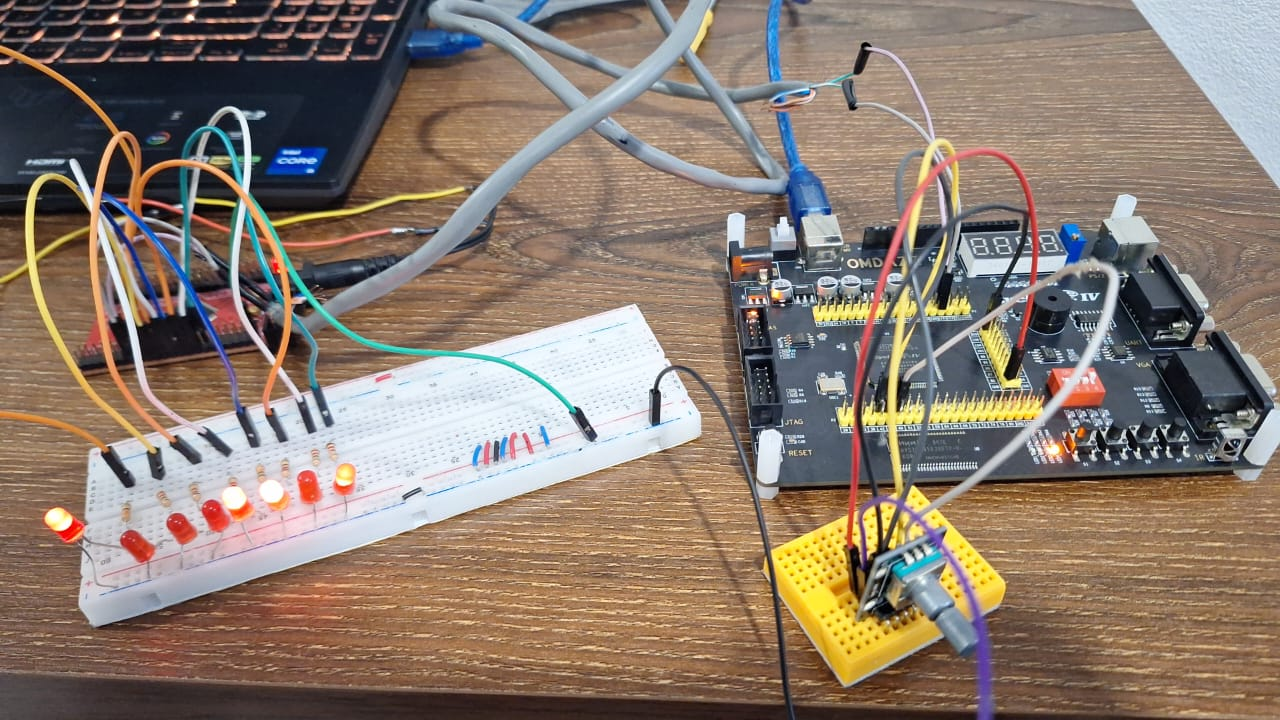
\includegraphics[width=0.5\linewidth]{Codigos/Encoder.png}
    \caption{Comunicación con protocolo RS232}\label{fig:rs232}
\end{figure}







\section{Conclusiones}
%! TEX root = C:\Users\osval\OneDrive - Instituto Politecnico Nacional\Codigos\Programacion\DLP\Practica_1\main.tex

\subsection*{Flores Oropeza Osvaldo}
    Durante la práctica note lo complejo que es diseñar etapas de potencia, ya sean de alimentación o de audio. Igualmente entendí la importancia de preparar con antelación los módulos necesarios para el correcto desarrollo de la práctica. \\
    En la primera actividad tuve problemas al darle significado físico a las salidas del sistema, esto debido a que lo ideal es que las salidas sean consecuencias del sistema diseñado. Esto es muy útil a la hora de diseñar sistemas de control, lo que nos ayudará durante la carrera. \\
    \textcolor{Amarillo}{\textbf{Frase:}} El \textcolor{Amarillo}{esfuerzo} sin objetividad y realidad no sirve. \\
    \textcolor{Amarillo}{\textbf{Metáfora:}} La metáfora habla de aceptación, cada persona es quien es no debería intentar ser alguien más, pero si debería intentar se mejor.

\subsection*{Ramírez Aguilar Víctor Saul}
    En esta practica se vio a simplicidad que puede llegar a tener el realizar algunas funciones basadas en circuitos de lógica secuencial y combinatoria con el uso de lenguajes VHDL y verilog para la programación de tarjetas FPGA, ya que no es muy diferente a otros lenguajes de programación donde podemos tener funciones para realizar tareas especificas, o el uso de vectores para el uso de lineas de datos como fue el caso del registro de 8 bits donde la función se realizo en pocas lineas de código lo que en un diseño con lógica combinacional física pudo haber requerido el uso de mas componentes. \\
    \textcolor{Amarillo}{\textbf{Frase:}} El \textcolor{Amarillo}{esfuerzo} trae buenas recompensas\\
    \textcolor{Amarillo}{\textbf{Lectura:}} Al ser estudiante de mecatronica creo que lo que quisiera transmitir al mundo seria compartir mi capacidad para tratar de resolver problemas de la vida cotidiana con soluciones tecnológicas.   
    
\subsection*{Reyes Lira Alejando}

    La práctica evidenció la capacidad y flexibilidad de los PLD para diseñar sistemas digitales diversos. Se inició con la descripción de una tabla de verdad en HDL, mostrando la eficiencia en la abstracción de lógica combinacional. Luego, se implementó un registro de 8 bits con flip-flops tipo D, destacando su importancia en el almacenamiento de datos. Posteriormente, se desarrolló un contador con salida a display de 7 segmentos, integrando conteo, decodificación e interfaz visual, esenciales en instrumentación. Finalmente, se aplicó el control de señales con la generación de sonidos de sirena, demostrando la interacción directa del PLD con el entorno. En conjunto, la práctica consolidó cómo estos dispositivos abarcan desde almacenamiento hasta generación de señales dinámicas, reafirmando su papel central en la tecnología digital.\\
    \textcolor{Amarillo}{\textbf{Frase:}} Enfoca tu \textcolor{Amarillo}{energia}, no en luchar contra lo que fuiste, sino en construir la persona que quieres llegar a ser.\\
    \textcolor{Amarillo}{\textbf{Metáfora:}} la metáfora nos enseña que la felicidad no proviene de lograr ser una buena imitación de otros, sino de un acto de valentía: mirar hacia nuestro interior, descubrir nuestra naturaleza única y abrazar nuestro propio y auténtico propósito, que es tan valioso como cualquier otro. 


%===========================BIBLIOGRAFIA=========================================


\nocite{*}
\bibliographystyle{IEEEtran}  % Estilo de la bibliografía en formato IEEE
\bibliography{Referencias}          

\end{document}
